\documentclass[14pt]{extreport}

% Шрифт
\usepackage[T2A]{fontenc}
\usepackage[utf8x]{inputenc}

% Языки и общие пакеты
\usepackage[english, russian]{babel}
\usepackage{csquotes}
% \usepackage{microtype}
\usepackage{graphicx}

% Подписи к рисункам (ГОСТ/положение: "Рисунок", по центру)
\usepackage[figurename=Рисунок, labelfont=bf, justification=centering]{caption}

% Выравнивание текста по ширине
\usepackage[newcommands]{ragged2e}
\usepackage{etoolbox}
\appto{\normalsize}{\justifying}

% Поля А4: левое 30 мм, правое 15 мм, верх/низ по 20 мм
\usepackage{geometry}
\geometry{
    a4paper,
    left=30mm,
    right=15mm,
    top=20mm,
    bottom=20mm
}

% Библиография по ГОСТ
\usepackage[
    backend=biber,
    style=gost-numeric,
    sorting=none,
    language=auto,
    autolang=other,
    movenames=false,
    bibencoding=utf8,
    parentracker=true,
    defernumbers=false,
    doi=false,
    eprint=false,
    isbn=false,
    url=false
]{biblatex}

% ГОСТ-настройки оформления библиографии
\DeclareFieldFormat[article]{title}{#1} % Название статьи без кавычек
\DeclareFieldFormat[book]{title}{#1}    % Название книги без кавычек

% Точки после каждого элемента библиографического описания
\renewcommand*{\newunitpunct}{\adddot\space}

% Файл библиографии
\addbibresource{literature.bib}

% Межстрочный интервал 1,5
\usepackage{setspace}
\onehalfspacing

% Абзацный отступ 1,25 см
\usepackage{indentfirst}
\setlength{\parindent}{1.25cm}

% Заголовки
\usepackage{titlesec}

% Увеличение tolerance для снижения underfull hbox в заголовках
\tolerance=10000

% Заголовок главы: 14 pt, по центру, без влияния setspace
\titleformat{\chapter}[display]
  {\normalfont\bfseries\centering\fontsize{14}{16}\selectfont}%
  {}{0pt}{}

\titlespacing*{\chapter}{0pt}{0pt}{12pt} % после заголовка чуть воздуха

% Заголовок параграфа (section): 14 pt, по центру
\titleformat{\section}
  {\normalfont\centering\fontsize{14}{16}\selectfont}%
  {\thesection}{1em}{}

% Исправленный spacing: вертикальный отступ сверху для избежания underfull hbox
\titlespacing*{\section}{0pt}{12pt}{6pt}


\begin{document}

adlkajsldkajs

\chapter{ОБЗОР ЛИТЕРАТУРЫ}

\section{Эволюционная динамика размеров и структуры бактериальных геномов}

Поиск взаимосвязи между последовательностью ДНК и её функциональным проявлением в бактериальной клетке является одним из ключевых направлений биологических исследований. Изучение данного вопроса позволяет раскрыть особенности механизмов реализации генетической информации у различных видов, а также сказать больше об их организации, образе жизни и эволюции.

Геном можно определить как <<программу жизни клетки>>, которая содержит в своей последовательности закодированную информацию не только продуктов биосинтеза, таких как, функциональные белки и различные типы РНК, но и другие <<структуры>>, которые выполняют широкий спектр функций. Например, сайты взаимодействия ДНК-связывающих белков, различные мотивы, оказывающие влияние на локальную топологию ДНК, а также автономные мобильные генетические элементы, способные к самостоятельной репликации и транспозиции в геноме (IS-элементы, транспозоны, CRISPR-повторы и т.д.). Разнообразие генетических элементов, характерных для геномов живых организмов подчеркивает взаимосвязь с эволюцией и адаптацией. Разделение множества элементов в геноме на <<существенное и несущественное>> в обеспечении жизнедеятельности клетки развивает концепция о минимальной клетке -- это теоретическая модель живой клетки, которая обладает минимальным набором генов (кодирующих наименьший из возможных набор функциональных белков и РНК) и способна к независимому росту и размножению в лабораторных условиях. Задача осложняется тем, что геномы живых организмов обладают свойством избыточности -- наличие в геноме дополнительных копий некоторых функциональных генов оставляет <<материал>> для дивергентной эволюции под <<натиском>> мутагенеза. Другое важное свойство -- <<буферность>> генома или <<его запас прочности>>, то есть существует порог объема мутаций, при внесении в структуру генома которых, функциональность живой клетки не страдает. Часть генных продуктов абсолютно необходима для обеспечения жизнеспособности клеток (такие как белки, кодируемые генами домашнего хозяйства), в то время как другая часть обеспечивает дополнительную селективную адаптивность к определенным факторам в зависимости от занимаемой экологической ниши.

В геномах бактерий широко распространена динамика расширения генного состава за счет различных эволюционных механизмов, например, в результате дубликации функциональных генов и последующей дивергентной эволюции копий в ходе приобретения мутаций. Патогенные микроорганизмы, находясь внутри организма хозяина пребывают в относительно более стабильной по условиям среде, чем свободно живущие виды, отсюда возникает положительный отбор на дубликаты генов, которые кодируют белки для усиления вирулентности. Полученные копии генов в результате дубликации могут <<разойтись>> по функции в результате дивергентной эволюции -- когда копии становятся отличны друг от друга в результате мутаций и выполнять разные функции. В ходе анализа с использованием биоинформатического конвейера SoDpipe \cite{wang2025deciphering} авторами было выявлено, что функция избыточных копий генов часто связана с повышением патогенности бактерий, более того, у патогенных штаммов, обладающих большей эволюционной дивергенцией от общих предков, был обнаружен более высокий коэффициент избыточности геномов (число избыточных генов, деленное на число белок-кодирующих), чем у не патогенных. Также, в ходе сравнительного биоинформатического анализа геномов патогенных микроорганизмов родов \textit{Klebsiella}, \textit{Escherichia} и \textit{Enterobacter} было выявлено, что изоляты, находящиеся в условиях селективного давления под воздействием антибиотиков и выделенные из организмов хозяинов (человек и сельско-хозяйственные животные), гораздо чаще имели дубликаты генов антибиотикорезистентности \cite{maddamsetti2024duplicated}.

Помимс процесса дубликации генов, в накоплении генетического материала участвует горизонтальный перенос генов (ГПГ) -- эволюционный механизм, заключающийся в переносе ДНК между организмами, которые не являются прямыми потомками друг друга. Гены, приобретенные в результате ГПГ, могут быть ассоциированы с вирулентностью и устойчивостью. Например, в изолятах патогенной бактерии \textit{Leptospira}, вызывающей лептоспироз, были найдены кластеры генов, приобретенные в результате ГПГ и дополняющие набор факторов вирулентности \cite{xu2016whole}. Геномные острова (genomic islands, GI) — кластеры генов, часто ассоциированные с tRNA-генами, способные интегрироваться в хромосому клетки-реципиента в результате горизонтального переноса. Среди них выделяют острова патогенности (pathogenicity islands, PAI), кодирующие специфические метаболические пути, токсины или системы секреции, обеспечивающие резкий рост вирулентности. Один из них — это остров высокой патогенности (high-pathogenicity island, HPI), кодирующий биосинтез металлофора йерсиниобактина (Ybt), характерен для представителей Enterobacteriaceae \cite{rakin2017ostrov} и распространяется в популяциях путем образования коинтегратов с конъюгативными плазмидами, такими как RP4.

Рассмотренные примеры иллюстрируют пластичность генного состава бактериальных клеток, направленную на накопление разнообразного генетического материала, однако, известен и обратный механизм, заключающийся в редукции генного состава. Свободно живущие виды подвергаются более широкому спектру воздействующих факторов внешней среды, отсюда необходимость в накоплении генетического материала с помощью ГПГ или других механизмов и сохранении разнообразия метаболических путей для обеспечения достаточной устойчивости и высокого адаптивного потенциала. У бактерий, чей <<образ жизни>> зависим целиком или только частично от метаболизма хозяина, геном может быть редуцирован. Редукция генома часто включает снижение GC (гуанин-цитозин) состава (AT-богатый геном), сокращение генного состава и утрата части метаболических путей (например, было показано, что у \textit{Mycoplasma pneumoniae} в геноме отсутствуют пути биосинтеза аминокислот, жирных кислот и холестерина \cite{himmelreich1996complete}). М

Представители класса \textit{Mollicutes}, являющиеся патогенами широкого спектра организмов, обладают существенно редуцированными геномами со среднем размером 1 Мб и часто выступают экспериментальной моделью минимальной клетки.

\section{Регуляция экспрессии генов в редуцированных геномах бактерий}

Экспрессия генов (транскрипция) - неотъемлемая часть многоступенчатого и сложного процесса реализации закодированной в геноме информации. Разнообразие механизмов координации уровня экспрессии генов формирует сложную сеть регуляции в постоянно меняющихся условиях среды, что обеспечивает высокий адаптивный потенциал организмам. Ключевым модулятором экспрессии большинства бактериальных генов является этап распознавания РНК-полимеразой промоторной области \cite{browning2004regulation}. Впервые в литературе промотор был определен как последовательность между оператором (регуляторная последовательность, примыкающая к генам и чувствительная к репрессору) и началом оперона \cite{jacob1964promoteur}. Промоторы часто характеризуют по наличию в последовательности ключевых элементов распознавания RNAP -- консервативных мотивов, расположение которых, как правило, зафиксировано в районе TSS (transcription start site - нуклеотид промотора, с которого
начинается считывание РНК). К таким мотивам относятся -35 элемент, -10 элемент (Pribnow box), UP-элемент, дискриминатор и так далее. На рисунке~\ref{fig:promoter_ecoli} изображена общая схема набора мотивов в промоторной области и их консенсусные последовательности для модельного организма \textit{E. coli}.

Набор специфичных мотивов и их консенсусные последовательности в промоторных областях разных видов бактерий существенно различаются. Например, последовательность элемента -10 у \textit{E. coli} преимущественно имеет вид 5'TATAAT, в то время как у бактерий вида \textit{Bacillus subtilis} консенсусная последовательность данного мотива выглядит как 5'CATAAT. Похожим образом у этих двух бактерий отличается друг от друга нуклеотидным составом -35 элемент промотора. Его консенсусная последовательность у \textit{E.coli} имеет вид 5'TTGACA, а у \textit{B.subtilis} -- 5'TTGACT \cite{lee1980nucleotide}.


Однако, было показано, что РНК-полимераза (RNAP) при отсутствии дополнительных факторов, например сигма-факторов или других регуляторов, способна инициировать начало транскрипции в местах разрывов ДНК (с ее концов) или на кольцевой двуцепочечной ДНК, то есть с последовательностей, отличных от промоторных областей \cite{vogt1969breaks, dausse1972interaction}. Таким образом, было показано, что наличие промотора необходимо для инициации биосинтеза транскриптов в определенных TSS (transcription start site - сайт начала транскрипции), а в процессе случайной транскрипции -- наличие промоторной области необязательно \cite{dausse1972interaction}. 




Экспрессия генов регулируется в ответ на изменение условий окружающей среды на каждом этапе, начиная с процесса инициации транскрипции, заканчивая стабильностью мРНК. Формирование обширного транскрипционного ответа играет решающее значение в выработке адаптивного потенциала клетками. Проблема заключается в определении -- какая часть из продуцируемых транскриптов клеткой является частью адаптации? Ведь масштабные изменения транскрипционного профиля в стрессовых условиях можно считать последствием дестабилизации работы регуляторных систем транскрипции, более того, не . Как было показано в одном из исследований, у бактерии \textit{Mycoplasmoides gallisepticum} \cite{mazin2014transcriptome} во время теплового шока количество мРНК в клетках сильно возрастает, в отличие от белков -- это означает, что только некоторая часть синтезируемых транскриптов будет частью адаптивного ответа (транслируемые транскрипты) к воздействию неблагоприятного фактора в виде высокой температуры. Однако, 


(далее про антисмысловую транскрипцию.... некодирующие РНК, цис-, транс- https://pmc.ncbi.nlm.nih.gov/articles/PMC7968456/)

Транскрипционный ответ в ходе адаптации к воздействию стрессовых факторов часто регулируется сродством промоторных областей к транскрипционным факторам (TF -- transcription factor). Переход между фазами роста или перенос неблагоприятных условий (окислительный, тепловой стресс, голод и т.д.) сопровождается накоплением клетками TF, которые координируют паттерн экспрессии генов, а следовательно и биологически активных продуктов, обеспечивая высокий адаптивный потенциал. Например, при наступлении стационарной фазы роста или при воздействии стрессовых факторов клетки \textit{Escherichia coli} накапливают сигма-фактор RpoS. Было показано, что активация его регулона приводит к повышению стрессоустойчивости клеток \cite{tanaka1993heterogeneity}.

Была обнаружена взаимосвязь между размером генома бактерий и количеством соответствующих транскрипционных факторов. В небольших геномах закодировано несколько TF, каждый из которых способен связывать большое количество участков, в то время как геномы большого размера содержат в своем составе много TF, которые связывают преимущественно собственные регуляторные участки (специализированные) \cite{galan2016transcription}. В особенности данные отличия заметны при сравнении видов бактерий, ведущих паразитический образ жизни со свободноживущими. Большинство представителей класса \textit{Mollicutes} ведут паразитический образ жизни, некоторые из них являются сапрофитами. Имеют редуцированный геном и обладают сокращенным набором TF, которые преимущественно опосредуют регуляцию экспрессии генов, участвующих во взаимодействиях с клетками хозяина и транспортом питательных веществ. В ходе сравнительного анализа наборов TF 50 видов класса \textit{Mollicutes} было установлено, что доля генов, кодирующих транскрипционные факторы, от общего числа генов в геноме, снижалась линейно с уменьшением размера генома, что отражено на рисунке~\ref{fig:TFs_mollicutes}. В итоге среднее количество TF для представителей класса \textit{Mollicutes} составляет 2,5\% от всех генов \cite{fisunov2016reconstruction}. Таким образом, упрощение (редукция) генома ведет к усложнению механизмов регуляции экспрессии генов, а именно обеспечивает систему <<регуляции без регуляторов>>. \textit{M. gallisepticum}, как представитель класса \textit{Mollicutes}, обладает сокращенным набором факторов транскрипции, по сравнению с близкородственной бактерией \textit{B. subtilis} \cite{moreno2006identification}. Однако, результаты исследований с транскриптомным профилированием показали наличие обширного транскрипционного ответа в результате воздействий внешних факторов среды у бактерий с редуцированным геномом и, соответственно, ограниченным набором TF. Транскриптомный анализ \textit{M. pneumoniae} в условиях теплового шока выявил экспрессию 564 из 676 исследованных (P < 0,001) генов (CDS), что составило 83\% от общего числа, что можно назвать обширным транскрипционным ответом \cite{weiner2003transcription}.

\begin{figure}[ht]
    \centering
    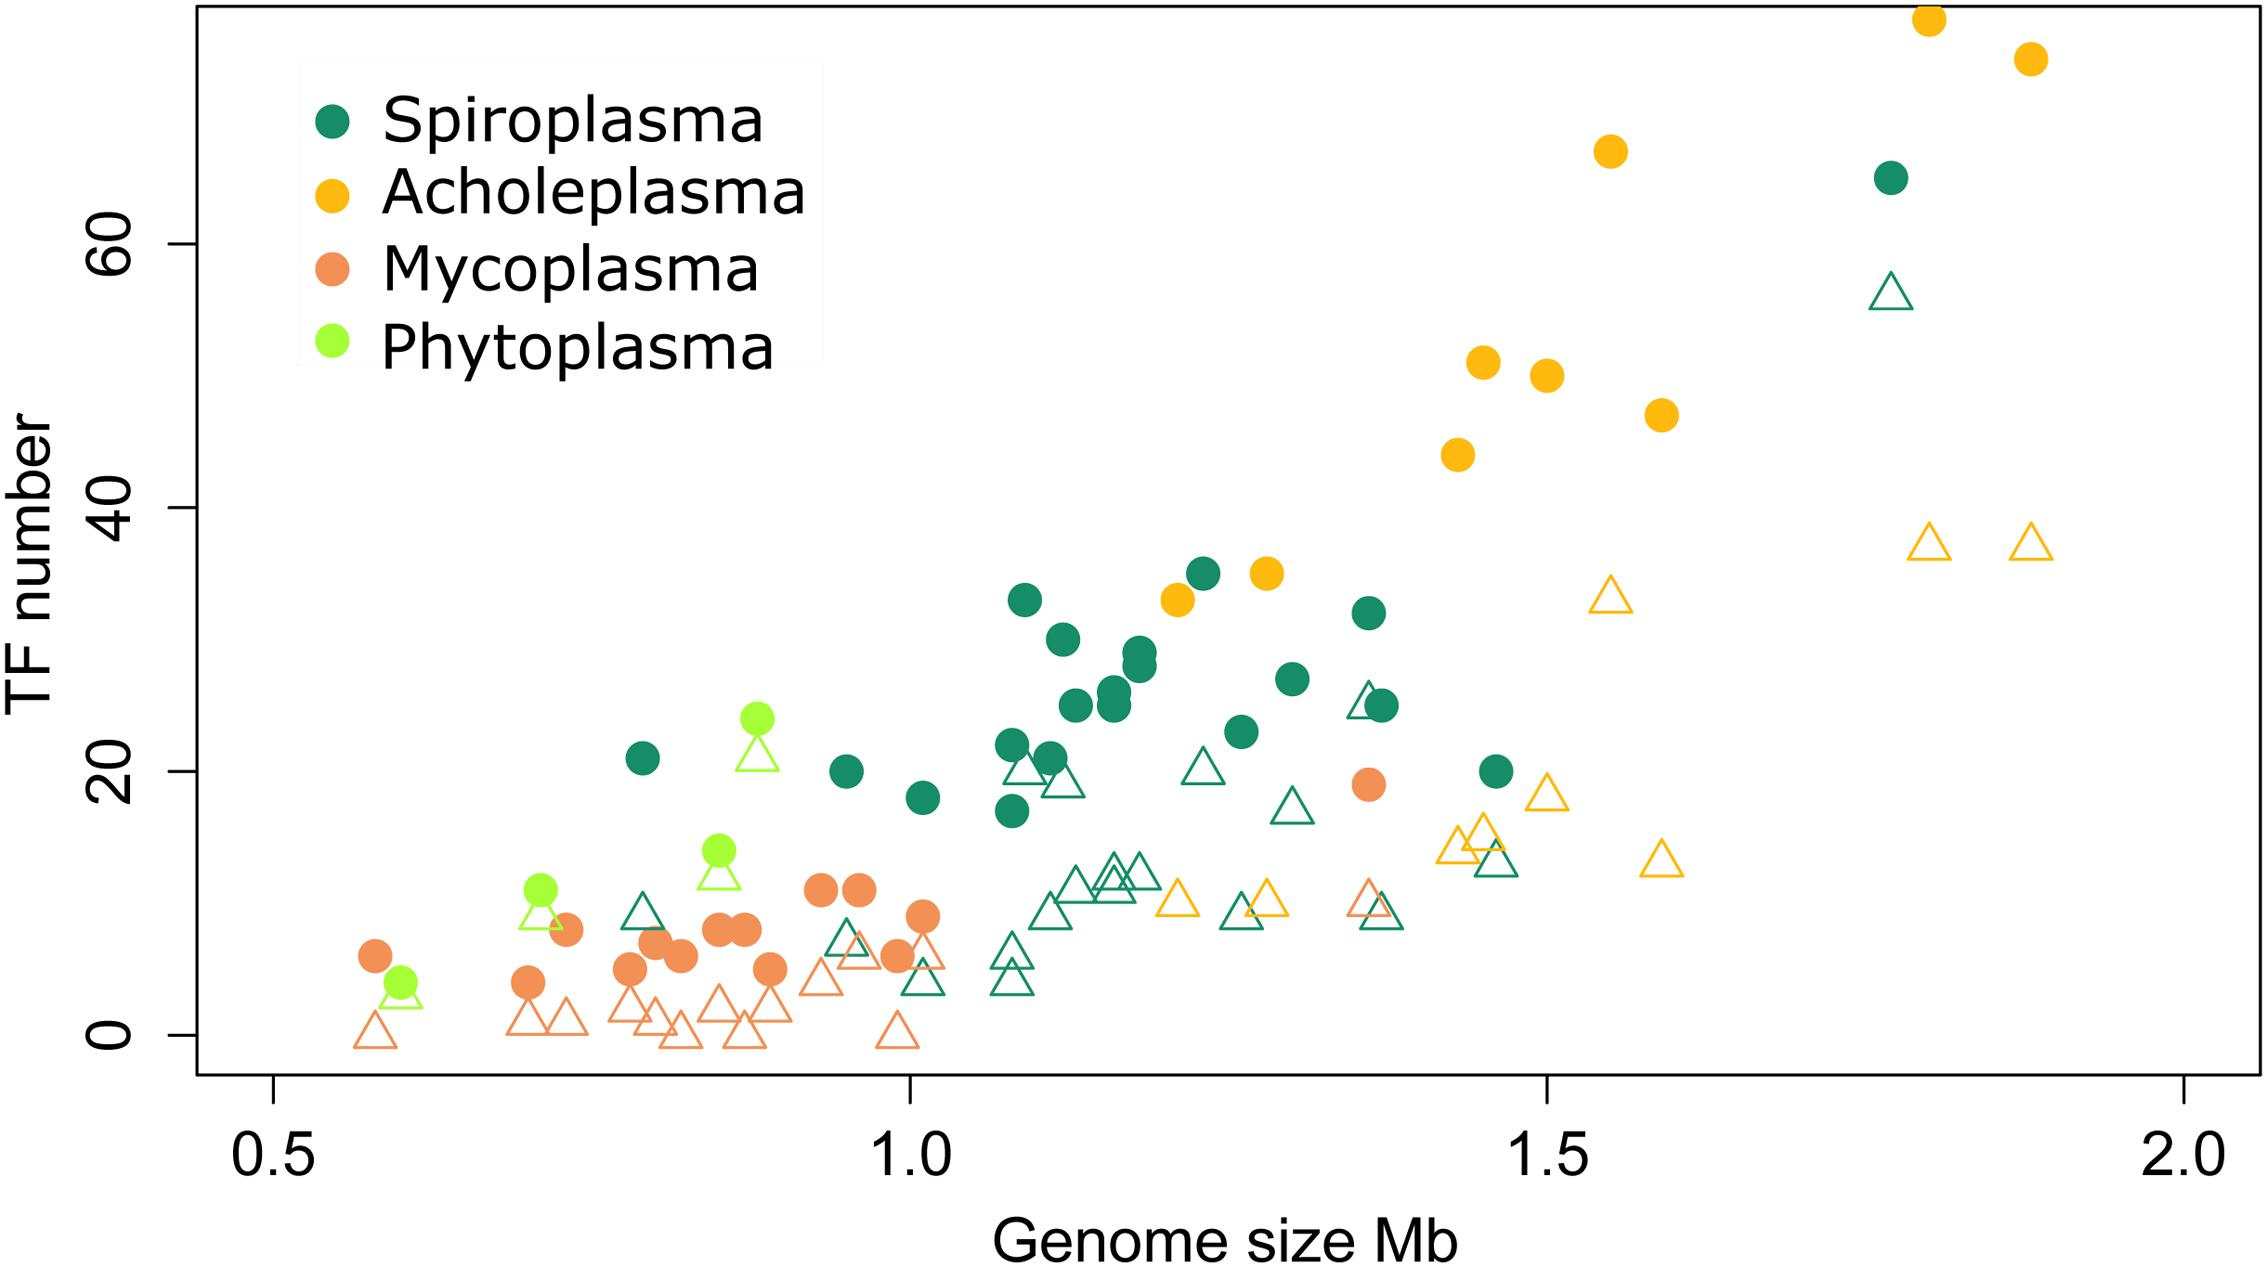
\includegraphics[width=0.7\linewidth]{TFs_mollicutes.jpg}
    \caption{Влияние редукции генома на количество транскрипционных факторов у \textit{Mollicutes} \cite{fisunov2016reconstruction}}
    \label{fig:TFs_mollicutes}
\end{figure}

Другим ключевым модулятором экспрессии большинства бактериальных генов является этап распознавания РНК-полимеразой промоторной области \cite{browning2004regulation}. Впервые в литературе промотор был определен как последовательность между оператором (регуляторная последовательность, примыкающая к генам и чувствительная к репрессору) и началом оперона \cite{jacob1964promoteur}. Однако, было показано, что РНК-полимераза (RNAP) при отсутствии дополнительных факторов, например сигма-факторов или других регуляторов, способна инициировать начало транскрипции в местах разрывов ДНК (с ее концов) или на кольцевой двуцепочечной ДНК, то есть с последовательностей, отличных от промоторных областей \cite{vogt1969breaks, dausse1972interaction}. Таким образом, было показано, что наличие промотора необходимо для инициации биосинтеза транскриптов в определенных TSS (transcription start site - сайт начала транскрипции), а в процессе случайной транскрипции -- наличие промоторной области необязательно \cite{dausse1972interaction}.

\section{Характеристика промоторных последовательностей бактерий}
Промоторы часто характеризуют по наличию в последовательности ключевых элементов распознавания RNAP -- консервативных мотивов, расположение которых, как правило, определено (зафиксировано) в районе TSS. К ним относится -35 элемент, -10 элемент (Pribnow box), UP-элемент, дискриминатор и так далее. На рисунке~\ref{fig:promoter_ecoli} изображена общая схема набора мотивов в промоторной области и их консенсусные последовательности для модельного организма \textit{E. coli}.

\begin{figure}[ht]
    \centering
    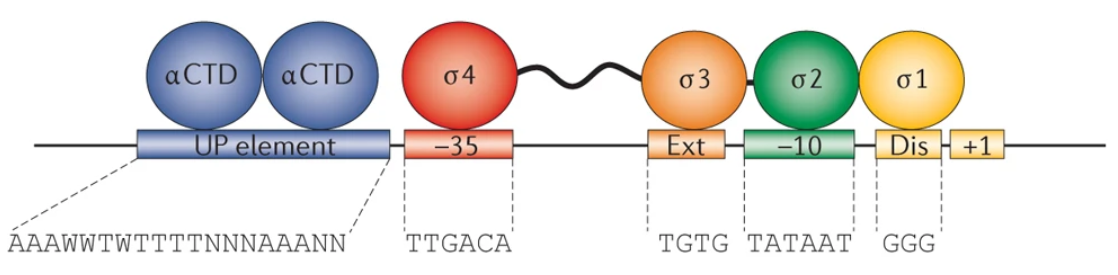
\includegraphics[width=0.7\linewidth]{Promoter_ecoli.png}
    \caption{Схема основных мотивов в структуре промотора \textit{Escherichia coli} и распознающие их субъединицы RNAP \cite{browning2016local}}
    \label{fig:promoter_ecoli}
\end{figure}

Набор специфичных мотивов и их консенсусные последовательности в промоторных областях разных видов бактерий существенно различаются. Например, последовательность элемента -10 у \textit{E. coli} преимущественно имеет вид 5'TATAAT, в то время как у бактерий вида \textit{Bacillus subtilis} консенсусная последовательность данного мотива выглядит как 5'CATAAT. Похожим образом у этих двух бактерий отличается друг от друга нуклеотидным составом -35 элемент промотора. Его консенсусная последовательность у \textit{E.coli} имеет вид 5'TTGACA, а у \textit{B.subtilis} -- 5'TTGACT \cite{lee1980nucleotide}. 

Промоторные области одного и того же организма различаются между собой набором структурных элементов или мотивов, степень соответствия консенсусу (сила промотора) которых напрямую влияет на их активность (частоту инициации транскрипции). Различные мотивы могут вносить в активность промотора как положительный (увеличивать частоту инициации и, как следствие, количество синтезируемых транскриптов), так и отрицательный вклад (так называемое залипание RNAP на промоторной области и удержание состояния закрытого комплекса). Например, у \textit{E. coli} в ходе сравнительного анализа 554 промоторных областей на наличие сходств в последовательностях был обнаружен пул промоторов, содержащих расширенный -10 элемент (добавлено 5'-TG-3'), а также более длинные спейсеры и отличный от консенсуса -35 элемент с несколькими ошибками \cite{mitchell2003identification}. Аналогично, было обнаружено, что отсутствие мотива -35 в промоторной области \textit{B.subtilis} может быть скомпенсировано наличием расширенного -10 элемента \cite{voskuil199816}. UP-элемент это мотив, расположенный перед -35 боксом, он состоит из области богатой аденином и тимином длиной около 30 нуклеотидов. В ходе инициации транскрипции с UP-эелементом взаимодействует альфа-субъединица RNAP (смотреть рисунок ~\ref{fig:promoter_ecoli}) \cite{ross1993third}. В совокупности соответствие структуры промоторной области оптимальной формуле (консенсусные мотивы, AT-состав, наличие других специфических регуляторных элементов и т.д.) опосредует повышение количества продуцируемых транскриптов промотором, а значит повышение его активности \cite{mitchell2003identification}. Существует множество подходов к предсказанию промоторных областей в прокариотических геномах, а также прогнозированию взаимосвязи между характеристиками последовательностей промоторов (генотип) и уровнем экспрессии контролируемых генов (фенотипическое проявление).

\section{Методы идентификации промоторных областей в прокариотических геномах \textit{in silico}}
Точное определение расположения промоторных областей в прокариотических геномах является одной из ключевых задач вычислительной биологии, поскольку это помогает в описании регуляции транскрипционных единиц бактерий -- оперонов. Более того, распределение промоторных областей по соответствующим им транскрипционным факторам позволяет определять генный состав регулонов TF и составлять регуляторные сети. Яркими примерами сборки системы регуляторных сетей бактерий являются: база данных для \textit{E. coli} K-12 RegulonDB \cite{santos2019regulondb}, DBTBS для \textit{B. subtilis} \cite{makita2004dbtbs}, также базы данных, включающие регуляторные сети для нескольких видов бактерий -- PRODORIC \cite{munch2003prodoric}, CoryneRegNet \cite{parise2020coryneregnet}.

Одним из подходов \textit{in silico}, используемых в предсказании промоторных областей на прокариотических геномах, являются алгоритмы, основанные на анализе гомологии регуляторных последовательностей, которые обладают сродством к соответствующим факторам транскрипции. Например, таким образом был проведен сравнительный анализ для последовательностей промоторов бактерий \textit{E. coli}, \textit{Salmonella typhimurium}, \textit{Yersinia pseudotuberculosis}. Авторы представили \textit{in silico} метод для прогнозирования сайтов связывания TF в промоторных областях ортологичных генов с предсказанием функциональной эволюции \cite{mustonen2005evolutionary}.

Принцип работы ряда алгоритмов заключается в применении позиционно-весовых матриц (PWM) различных мотивов регуляторных областей для сканирования геномов бактерий. С использованием данного подхода были выявлены высококонсервативные мотивы в промоторных областях генов \textit{Lactobacillus plantarum}, часть из которых относится к регулируемым сигма-фактором RpoD \cite{todt2012genome}. Схожим образом, с использованием алгоритма position-correlation scoring matrix (PCSM) были предсказаны сайты связывания сигма-фактора RpoD в геноме \textit{E. coli} K-12 \cite{li2006recognition}. Однако, не всегда в промоторных последовательностях можно найти высококонсервативные мотивы, широко представленные у большинства бактерий. У некоторых видов регуляторные области обладают чуть большей вариативностью. Так, в геноме \textit{M. gallisepticum} отсутствует выраженный бокс -35 (дегенерация промотора), по сравнению с \textit{A. laidlawii} и \textit{S. melliferum}, помимо этого, былы обнаружены тандемные промоторы, состоящие из двух повторяющихся элементов -10 с коротким спейсером либо перекрывающимися \cite{fisunov2016reconstruction}.

Было установлено, что истинные промоторы (продуктивные) --- результатом инициации транскрипции с таких промоторов является транслируемый далее транскрипт, в геноме часто окружены мотивами с промотороподобным сигналом, которые конкурируют за связывание с RNAP \cite{huerta2003sigma70}. Более того, шумных мотивов в геномах в разы больше, чем истинных -- это часто приводит к ложноположительным результатам предсказаний алгоритмами промоторных областей \cite{hertz19962, horton1992assessment}. К создающим шум промотороподобным последовательностям относят мотивы соответствующие -10 элементу (Pribnow box), но расположенные изолированно от TSS -- tssRNA, которые приводят к биосинтезу не функциональных транскриптов длиной около 40 нуклеотидов \cite{yus2012transcription}. Для генома бактерии \textit{Mycoplasma pneumoniae} с использованием алгоритма машинного обучения Random forest был создан классификатор для предсказания промоторных областей и их разделения на истинные, абортивные и промотороподобные регуляторные последовательности \cite{llorens2015distinguishing}. 

%% \defbibheading{bibliography}[\bibname]{%
%%   \chapter*{СПИСОК ЛИТЕРАТУРЫ}%
%%  \markboth{СПИСОК ЛИТЕРАТУРЫ}{СПИСОК ЛИТЕРАТУРЫ}%
%% }
%%\printbibliography[heading=bibliography]
%%\addcontentsline{toc}{chapter}{СПИСОК ЛИТЕРАТУРЫ}


\end{document}